\documentclass[10pt,a4paper]{article}
\usepackage[utf8]{inputenc}
\usepackage{hyperref}
\usepackage{listings}
\usepackage{color}
\usepackage{graphicx}
\definecolor{dkgreen}{rgb}{0,0.6,0}
\definecolor{gray}{rgb}{0.5,0.5,0.5}
\definecolor{mauve}{rgb}{0.58,0,0.82}

\lstset{frame=tb,
  language=sh,
  aboveskip=3mm,
  belowskip=3mm,
  showstringspaces=false,
  columns=flexible,
  basicstyle={\small\ttfamily},
  numbers=none,
  numberstyle=\tiny\color{gray},
  keywordstyle=\color{blue},
  commentstyle=\color{dkgreen},
  stringstyle=\color{mauve},
  breaklines=true,
  breakatwhitespace=true,
  tabsize=3
}

\author{Josué Alvarez}
\title{Simso web - Developper Documentation}
\begin{document}
\maketitle
\newpage
\section{Preamble}
This document is a non-exhaustive developer documentation, whose goal is to help future maintainers of the simso-web application to get started with the code. 
This document is written with the assumption that the developper is using an UNIX environment.

\section{Getting Started}
\paragraph{Introduction}
Simso web is a graphical interface built on top of simso. It runs as a full-client application (no server-side) written in javascript, and uses PypyJS (a javascript implementation of \href{"http://www.pypy.org/"}{Pypy}) to run Python in order to execute simso.
The main frameworks/tools used for the front-end development are \href{"https://angularjs.org/"}{Angular JS} and \href{"http://getbootstrap.com/"}{Bootstrap}.

\subsection{Getting the code}
The code is available on github here : https://github.com/MaximeCheramy/simso-web. 
As simso-web embbeds its own version of simso, it is included in the form of a git submodule.

To setup your working copy, you have to run the following commands :
\begin{lstlisting}
git clone https://github.com/MaximeCheramy/simso-web.git
cd simso-web/submodules/simso
git submodule init
git submodule update
\end{lstlisting}

\subsection{Architecture}
\paragraph{Overview}
The project is composed of 3 major components :
\begin{itemize}
\item The HTML / Javascript / AngularUI front-end.
\item Simso : the component used to run the simulation.
\item The python bridge between Simso and the Javascript application.
\end{itemize}

\begin{figure}[h]
\centering
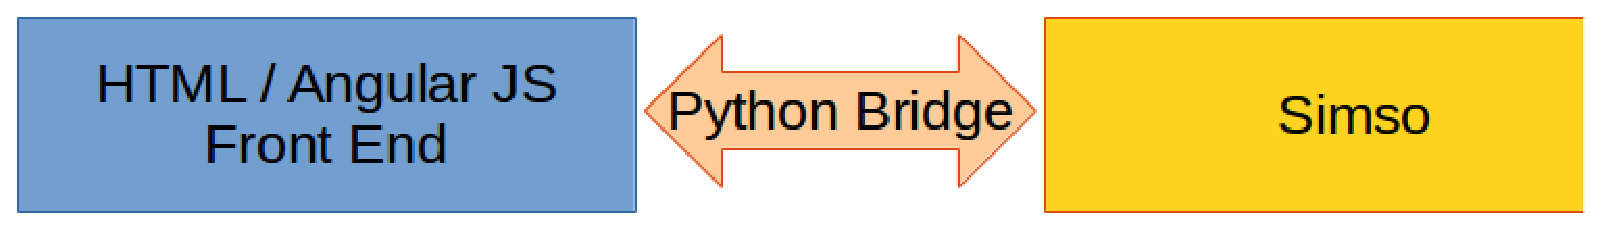
\includegraphics[scale=0.50]{figure1.eps}
\caption{Simso web's major components}
\end{figure}

\paragraph{Use case}
In order to understand the structure of the code, we are going to introduce a typical simso-web use case :
\begin{enumerate}
\item The user sets up a configuration on the configuration view.
\item The user clicks on the "Run" button
	\begin{itemize}
	\item A python configuration script is created using the parameters in the configuration view (file js/controlers/config-controler.py). This script is then executed and creates a python 'Configuration' object.
	\item The 'run()' method of the Bridge is called (py/simso-bridge.py) and launches the Simso simulation.
	\item Once this is done, a variable containing the results of the simulation is created in a way it can be read by the javascript application.
	\end{itemize}
\item The user clicks the "Results" button : the results are now displayed. Some python functions (in py/simso-bridge.py) are used to aggregate results.
\end{enumerate}

\paragraph{The HTML / Javascript / Angular UI front-end}


The front end is built upon the MVC architecture.
\begin{itemize}
\item The Model : the model files are contained within the js/services/ directory. They are called 'services'. The main services are :
	\begin{itemize}
	\item conf-service.js : contains all the data related to the Configuration of the simulation. That data is going to be used to generate the configuration script.
	\item pypy-service.js : contains all the code related to the initialisation of the virtual machine.
	\end{itemize}
\item The Views : the view files are contained in the partial/ folder. They are HTML files. There are 2 main views : 
\begin{itemize}
\item The Configuration view is the place where the user can setup the simulation parameters.
\item The Results view is the place where the user can see the simulation's results once it has been run.
\end{itemize}

\item The Controlers : the controlers are located within the js/controlers/ directory. 

\end{itemize}


\pagebreak

\paragraph{The bridge}
The bridge is responsible for passing configuration to simso, gathering results and passing them back to javascript.
\begin{figure}[h]
\centering
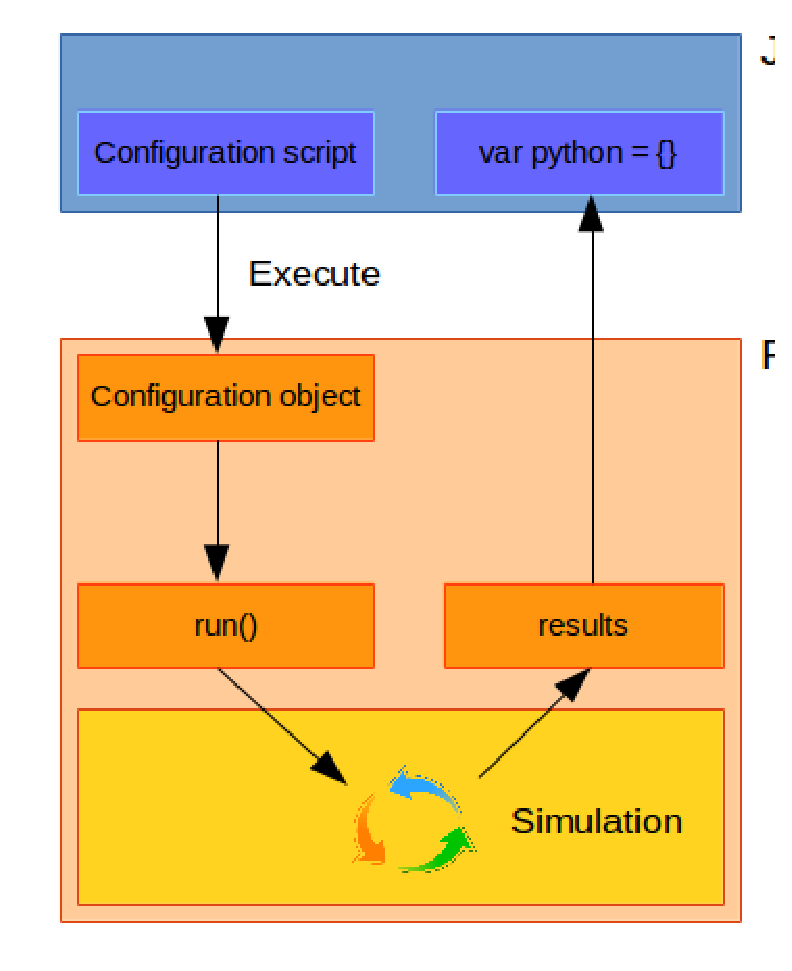
\includegraphics[scale=0.50]{figure2.eps}
\caption{The python bridge}
\end{figure}


\paragraph{Simso}
Simso is integrated in simso-web as a submodule. Simso's documentation is available here : \href{"http://homepages.laas.fr/mcheramy/simso/doc"}{http://homepages.laas.fr/mcheramy/simso/doc}.

\end{document}

